\section{API Design and Implementation}

\subsection{API style and conventions}

PizzaHUST exposes a REST-style HTTP API under the \texttt{/api} namespace. The backend publishes an OpenAPI description at \texttt{/api/openapi.json}, and the current frontend uses generated TypeScript types derived from that contract. JSON is the default data format for request and response bodies, while multipart upload is reserved for specific cases such as image uploads and CSV import.

Several contract conventions are used consistently:

\begin{itemize}
    \item money values are represented as integer VND amounts;
    \item timestamps use ISO 8601 date-time formatting;
    \item internal database-backed resources use integer identifiers;
    \item public guest order tracking uses an order code rather than exposing internal IDs.
\end{itemize}

These conventions reduce ambiguity across the frontend, backend, and testing layers.

\subsection{Authentication and security model}

The API is designed for a browser-based session workflow rather than token-only SPA authentication. Authenticated access depends on a signed session cookie managed by the backend. The frontend API client sends requests with browser credentials enabled and automatically attaches a CSRF token header for mutating requests when the token is present in cookies.

Role-restricted actions are enforced in the backend through dependency-based guards. This means the same API host can expose:

\begin{itemize}
    \item public routes for browsing, quoting, and some guest-facing order functions;
    \item customer-only routes for account and loyalty behavior;
    \item admin-only routes for catalog, order, customer, settings, and reporting management;
    \item kitchen-only routes for operational queue actions;
    \item externally callable webhook routes protected by message authentication.
\end{itemize}

\subsection{Error model}

PizzaHUST does not return arbitrary error shapes. Non-success responses are normalized into an error envelope containing:

\begin{itemize}
    \item an application-level error code;
    \item a human-readable message;
    \item optional structured details;
    \item the current request ID.
\end{itemize}

This is important for two reasons. First, frontend code can respond consistently to expected failures such as validation errors, unauthorized access, or business-state conflicts. Second, the request ID allows debugging and log correlation across the backend boundary.

The current backend error handling maps raw HTTP failures into a closed contract-level code set, including validation, authentication, authorization, conflict, rate limiting, and delivery-upstream errors.

\subsection{API surface by module}

The current OpenAPI file contains 63 documented paths. Table~\ref{tab:api-surface} groups them by functional area.

\begingroup
\small
\setlength{\LTpre}{0.4em}
\setlength{\LTpost}{0.8em}
\captionof{table}{Current API surface grouped by module}\label{tab:api-surface}
\begin{tabular}{L{0.19\linewidth} L{0.10\linewidth} L{0.18\linewidth} L{0.43\linewidth}}
\toprule
\textbf{API group} & \textbf{Paths} & \textbf{Typical access} & \textbf{Main purpose} \\
\midrule
Health & 1 & Public & Service health check for runtime readiness. \\
Configuration & 3 & Public & Read delivery, loyalty, and business-setting values needed by the frontend. \\
Catalog & 3 & Public & Browse categories and item list/detail data. \\
Combos & 2 & Public & Browse combo list and combo detail data. \\
Cart & 5 & Public or session-backed & Quote, retrieve, and manage cart state. \\
Orders & 5 & Mixed & Place orders, track orders, and retrieve customer order history. \\
Authentication & 4 & Mixed & Register, login, logout, and inspect/update current account state. \\
Loyalty & 1 & Customer session & Return loyalty summary data. \\
Administrator & 33 & \texttt{admin} role & Manage catalog, options, combos, customers, orders, reports, import, and settings. \\
Kitchen & 5 & \texttt{kitchen} role & View operational order data and perform kitchen-side actions. \\
Webhooks & 1 & HMAC protected & Accept external delivery-status callbacks. \\
\bottomrule
\end{tabular}
\endgroup

This grouping shows that the administrative surface is the largest part of the API. That is consistent with the system's dual nature as both a customer storefront and a store-operation platform.

\subsection{Representative endpoint behavior}

Representative endpoints are more useful than a raw endpoint list because they illustrate how the API applies validation, authorization, and business rules in practice.

\begingroup
\small
\setlength{\LTpre}{0.4em}
\setlength{\LTpost}{0.8em}
\captionof{table}{Representative endpoint behavior}\label{tab:representative-endpoints}
\begin{tabular}{L{0.20\linewidth} L{0.32\linewidth} L{0.39\linewidth}}
\toprule
\textbf{Method and path} & \textbf{Purpose} & \textbf{Important behavior} \\
\midrule
\texttt{GET /api/items/\{id\}} & Return one active menu item. & Returns item details and enabled option groups for customer-side customization; inactive items are not treated as valid public resources. \\
\texttt{POST /api/cart/quote} & Compute an authoritative preview quote. & Deduplicates selected option IDs, validates option rules and combo selections, resolves live prices from the database, and optionally checks delivery-area rules. \\
\texttt{POST /api/orders} & Place a COD order from cart state. & Converts validated cart lines into a durable order, creates an order code, persists item snapshots, and rejects invalid cart or address state. \\
\texttt{POST /api/auth/login} & Start an authenticated customer/admin/kitchen session. & Validates credentials, enforces account restrictions, sets session and CSRF cookies, and uses controlled error handling for authentication failure. \\
\texttt{POST /api/admin/orders/\{id\}/retry-dispatch} & Retry delivery handoff for an exception order. & Requires administrative access, permits only valid retry states, and preserves consistency if the upstream delivery provider fails again. \\
\texttt{POST /api/kitchen/orders/\{id\}/mark-ready} & Move a prepared order toward dispatch. & Enforces kitchen authorization, validates workflow state, and may produce either \texttt{ReadyForDispatch} or a retryable handoff-failure state depending on delivery-port outcome. \\
\texttt{POST /api/webhooks/delivery} & Accept courier status synchronization. & Requires HMAC validation, uses idempotency protection, maps provider states into internal order-state rules, and records tracking updates only for valid transitions. \\
\bottomrule
\end{tabular}
\endgroup

\subsection{Representative request/response patterns}

The design of the API can also be seen in the structure of a few core request/response patterns:

\begin{itemize}
    \item \textbf{Quote requests} accept candidate cart lines and optional address information, but never trust the client to supply price values.
    \item \textbf{Order placement requests} collect delivery information and optional notes, then transform session-backed cart state into durable business records.
    \item \textbf{Administrative mutation requests} rely on session role checks plus CSRF protection, reflecting the browser-based staff UI model.
    \item \textbf{Webhook requests} invert the normal user-driven pattern by accepting externally initiated state changes under strict signature validation.
\end{itemize}

These patterns show that the API is designed around business workflows rather than only CRUD-style resource manipulation.

\subsection{Contract generation and drift control}

Contract discipline is one of the strongest technical aspects of the current PizzaHUST implementation. The backend exports the OpenAPI document automatically, and the project verification pipeline checks that the committed contract file remains synchronized with generated output. The frontend then regenerates \texttt{lib/api/types.ts} from the OpenAPI description and checks that the generated type file has not drifted.

This workflow provides two important benefits:

\begin{itemize}
    \item it reduces the risk that frontend request/response assumptions silently diverge from backend behavior;
    \item it turns the API specification into a maintained artifact rather than a document that becomes stale after implementation changes.
\end{itemize}

\subsection{Interaction-flow diagrams}

The existing sequence diagrams are still useful as high-level illustrations of the main order-processing interactions. They show the coordination between browsing, quotation, checkout, kitchen progression, delivery handoff, and tracking, not just isolated endpoint calls.

\begin{figure}[htbp]
    \centering
    
\includegraphics[page=2,width=0.92\textwidth,height=0.68\textheight,keepaspectratio]{latex_report/figures/order_flow_implemented.pdf}
    \caption{Implemented quotation-focused API interaction flow}
    \label{fig:order-flow-quotation}
\end{figure}

\begin{figure}[htbp]
    \centering
    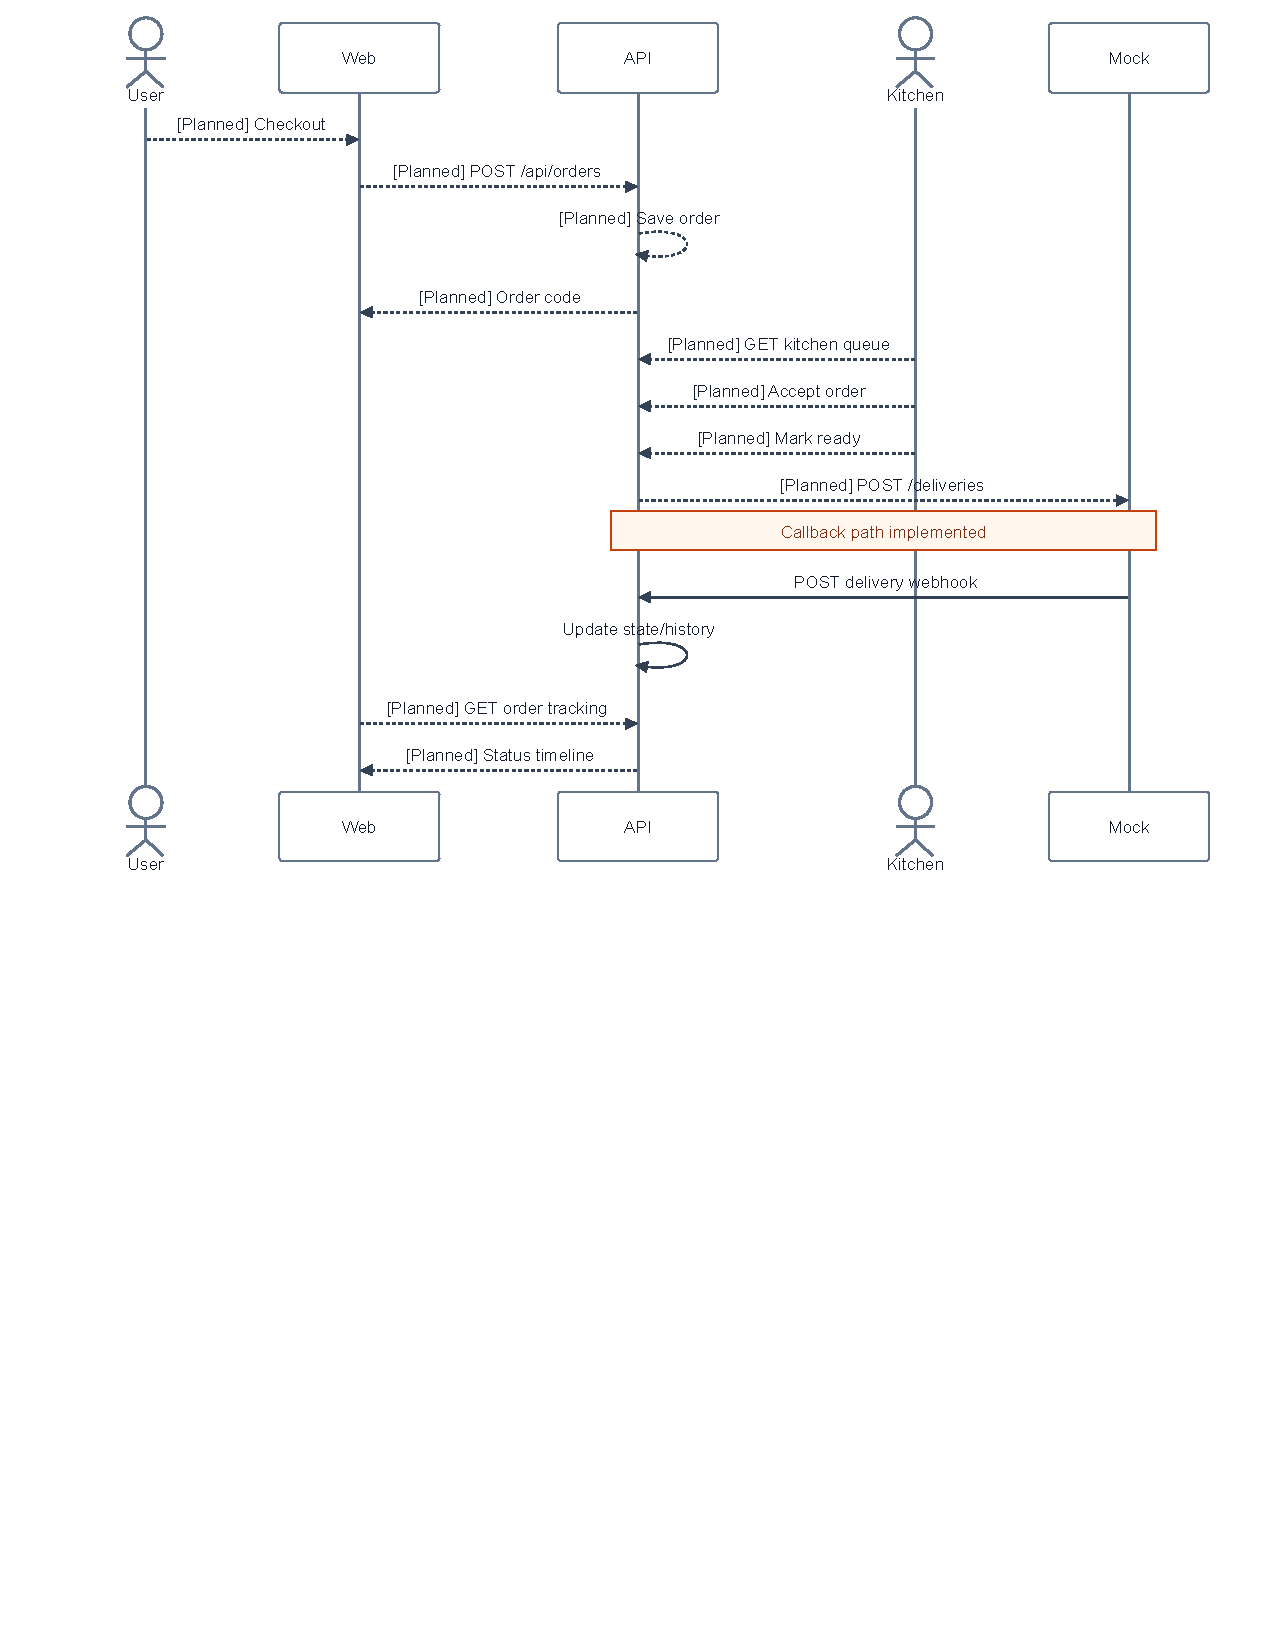
\includegraphics[width=\textwidth,height=0.78\textheight,keepaspectratio,trim=55 368 25 5,clip]{latex_report/figures/order_flow_delivery_flow.pdf}
    \caption{Broader order-processing and delivery-tracking interaction flow}
    \label{fig:order-flow-delivery-tracking}
\end{figure}

The first diagram aligns more directly with already implemented quotation behavior, while the second represents the broader end-to-end workflow view.

\subsection{API coverage}

This API section describes the current implementation and the full contract surface. The repository contains substantial operational endpoints for catalog browsing, pricing, order placement, administrative management, kitchen actions, customer-account features, loyalty, and delivery synchronization. The report therefore presents the API as a strong, structured contract surface that is now aligned with the completed product scope.
